\chapter{Methods}
In order to benefit directly from the FINN code, the GitHub repository created by Karlbauer et al. \cite{karlbauer2021composing} was forked. The methods needed in this work were implemented in the structure provided by the FINN framework. Other equations which are already implemented in the FINN framework (Allen-Cahn, Burgers, etc.) are not affected by this work.\\
\section{Underlying Equations}
To model the 1D transport of a substance through soil, water flow and solute transport have to be considered:\\
Water flow in soil can be described with the Richards equation \cite{Richards1931Nov}
\begin{equation}
    \frac{\partial \theta (h)}{\partial t} = \frac{\partial}{\partial x} \biggl [K(h)\biggl(\frac{\partial h}{\partial x} +1\biggr)\biggr] -S,
    \label{eq:richard}
\end{equation}
where $x$ is the vertical coordinate positive upward $[L]$, $t$ is the time $[T]$, $h$ is the pressure head $[L]$, $\theta$ is the volumetric water content $[L^3 L^{-3}]$, $S$ is a source or sink term $[T^{-1}]$ and $K(h)$ is the unsaturated hydraulic conductivity function.\\
\\
Numerical models for solute transport including sorption are based on the AD equation
\begin{equation}
    \frac{\partial \theta c}{\partial t} + \rho \frac{\partial s}{\partial t} = \frac{\partial }{\partial x} \left(\theta D \frac{\partial c}{\partial x} \right) - \frac{\partial qc}{\partial x},
    \label{eq:ad}
\end{equation}
where $c$ is the concentration of the dissolved substance $[M L^{-3}]$, $s$ is the mass specific sorbed concentration $[M M^{-1}]$, $q$ is the Darcy flux $[L T^{-1}]$ and $D$ is the dispersion coefficient. $D$ is the combination of the hydrodynamic and the effective molecular diffusion coefficient \cite{Scheidegger1961Oct}, which is calculated by:
\begin{equation}
    D = \alpha_lv + D_e,
    \label{eq:d_etodisp}
\end{equation}
where $\alpha_l$ is the longitudinal dispersivity $[L]$, $D_e$ the effective molecular diffusion coefficient $[L^2 T^{-1}]$, and $v$ $[LT^{-1}]$ the seepage, or effective velocity. On the present Darcy scale, the effective velocity is assumed to be constant over space. However, due to the heterogeneity of the porous medium, local scattering, dilution or mixing of solutes may occur. To account for this, eq. \ref{eq:d_etodisp} contains the velocity-proportional dispersion term called hydrodynamic dispersion \cite{Scheidegger1961Oct}.
The effective velocity $v$ is calculated by
\begin{equation}
    v = \frac{q}{n_e},
    \label{eq:darcytov}
\end{equation}
where $q$ is again the Darcy flux $[LT^{-1}]$ and $n_e$ $[-]$ the effective porosity.\\
During the simulations and experiments, a saturated water flow was set. Thus, the water fraction $\theta$ stayed constant for the entire simulation time and corresponds the effective porosity $n_e$. Therefore, the Richards equation \ref{eq:richard} need not be solved and $\theta$ can be pulled out of time and space derivatives in the AD equation \ref{eq:ad}. Dispersion coefficient $D$ and Darcy flux $q$ are also spatially independent and can be pulled out. Dividing by $n_e$ ($n_e \neq 0$) and using eq. \ref{eq:darcytov} yields
\begin{equation}
    \frac{\partial c}{\partial t} + \frac{\rho}{n_e} \frac{\partial s}{\partial t} = D \frac{\partial^2 c}{\partial x^2} - v\frac{\partial c}{\partial x}.
    \label{eq:ad2}
\end{equation}
\\
Using the 2SS model, the sorption process is divided into two parts
\begin{equation}
    s = s_e + s_k,
\end{equation}
where $s_e$ $[M M^{-1}]$ is an instantaneous equilibrated sorption process, which is describable by a sorption isotherm, $s_k$ $[M M^{-1}]$ is modeled as a first-order kinetic rate process. The term $\frac{\rho}{n_e} \frac{\partial s}{\partial t}$ in \ref{eq:ad2} thus expands to
\begin{equation}
        \frac{\partial c}{\partial t} + \frac{\rho}{n_e} \frac{\partial s_e}{\partial t} + \frac{\rho}{n_e} \frac{\partial s_k}{\partial t} = D \frac{\partial^2 c}{\partial x^2} - v\frac{\partial c}{\partial x}.
    \label{eq:ad2ss}
\end{equation}
In this work, the Freundlich sorption isotherm \cite{Freundlich1907Oct} was used for calculation of $s_e$
\begin{equation}
s_e = fk_dc^{\beta}
    \label{eq:freundlich}.
\end{equation}
$f$ $[-]$ is the fraction of sites that are expected to be in equilibrium with the liquid phase, $k_d$ $[L^3 M^{-1}]$ is the Freundlich constant, and $\beta$ $[-]$ the Freundlich exponent.\\
The first-order kinetic velocity process is modeled by
\begin{equation}
    \frac{\partial s_k}{\partial t} = \alpha_k ((1-f)k_dc^{\beta} - s_k),
    \label{eq:rate_process}
\end{equation}
where $\alpha_k$ is the first-order rate constant $[T^{-1}]$. The equation can be interpreted: A high dissolved concentration and a low kinetically sorbed concentration lead to a positive value on the right-hand side ($\alpha_k > 0$). Thus, the time derivative of $s_k$ is positive and an increase in $s_k$ can be observed for the next time step. The same reasoning can be done for a decrease of $s_k$.\\
Eq. \ref{eq:rate_process} has the analytical solution
\begin{equation}
    s_k(t) = \mathcal{K}e^{-\alpha_k t} + (1-f)k_dc(t)^{\beta} \qquad \mathcal{K} \in \mathbb{R}.
    \label{eq:sol_rate_process}
\end{equation}
If equilibrium is reached with the liquid-phase concentration ($t \rightarrow \infty$), the originally kinetically sorbed concentration can then be calculated with
\begin{equation}
    s_k(t) = (1-f)k_dc(t)^{\beta}.
\end{equation}
The sorption process is then describable by the sorption isotherm
\begin{equation}
    s(t) = s_e(t) + s_k(t) = fk_dc(t)^\beta + (1-f)k_dc(t)^\beta = k_dc(t)^\beta.
\end{equation}\\
It holds for eq. \ref{eq:freundlich} because of the chain rule \ref{eq:chain_rule}
\begin{equation}
    \frac{\partial s_e}{\partial t} = fk_d\beta c^{\beta-1}\cdot\frac{\partial c}{\partial t},
    \label{eq:s_e_der}
\end{equation}
since $f$ and $k_d$ are time-independent. With eq. \ref{eq:s_e_der} it holds for eq. \ref{eq:ad2ss}:
\begin{align}
    \frac{\partial c}{\partial t} + \frac{\rho}{n_e} fk_d\beta c^{\beta-1}\cdot\frac{\partial c}{\partial t} + \frac{\rho}{n_e} \frac{\partial s_k}{\partial t} &= D \frac{\partial^2c}{\partial x^2} - v\frac{\partial c}{\partial x}\nonumber\\
    &\Leftrightarrow \nonumber\\
    \frac{\partial c}{\partial t} \cdot \underbrace{\biggl(1 + \frac{\rho}{n_e} fk_d\beta c^{\beta-1}\biggr)}_{=:\:R(c)} + \frac{\rho}{n_e} \frac{\partial s_k}{\partial t} &= D \frac{\partial^2c}{\partial x^2} - v\frac{\partial c}{\partial x}.
    \label{eq:ad2ss_t}
\end{align}
$R$ represents the retardation factor resulting from instantaneous sorption.
\section{Solving the Transport Equation with Finite Differences}
All models in the FINN framework contain a FD solver to solve the underlying equations to generate synthetic training or test data. Thus, a FD solver for the AD equation including the 2SS model (AD2SS) was implemented too. To solve eq. \ref{eq:ad2ss_t} with different settings separately from the source code, in contrast to other FD solvers in the FINN framework, a \texttt{parmas} .json-file was created, where all parameters can be specified. Parameter names mentioned in the following always refer to the described \texttt{params} .json-file. For reproducibility an exemplary file can be found on GitHub \cite{FINN_fork}.\\
\\
In particular, on equidistant 1D grids, classical FD solvers are an intuitive way to solve PDEs. Based on Taylor's theorem, difference quotients are used to approximate derivatives of various orders.
\subsection{Spatio-temporal Discretization}
Let $X_{LENGTH}$ $[L]$ be the length of the considered 1D domain $\Omega_x$ with $X_{STEPS} \in \mathbb{N}$ lattice points arranged equidistantly. Then for the lattice width $dx$ $[L]$ holds
\begin{equation}
    dx := \frac{X_{LENGTH}}{X_{STEPS} - 1},
    \label{eq:dx}
\end{equation}
or for the discretized simulation space $\Omega_x$
\begin{equation}
    \Omega_x := \{0, 1\cdot dx, 2\cdot dx, ... , (X_{STEPS}-2)\cdot dx, X_{LENGTH}\}.
\end{equation}
Analogously, if $T_{MAX}$ $[T]$ is the simulation time with $T_{STEPS} \in \mathbb{N}$ simulation time steps arranged equidistantly, then for the simulation time step $dt$ $[T]$ holds
\begin{equation}
    dt := \frac{T_{MAX}}{T_{STEPS} - 1},
    \label{eq:dt}
\end{equation}
or for the discretized simulation time $\Omega_t$
\begin{equation}
    \Omega_t := \{0, 1\cdot dt, 2\cdot dt, ... , (T_{STEPS}-2)\cdot dt, T_{MAX}\}.
\end{equation}
Let $c: \Omega_x \, \times \, \Omega_t \rightarrow \mathbb{R}^{X_{STEPS}}$ be the unknown volume specific concentration of PFOS dissolved in water with the spatial indexing for any fixed but arbitrary $t \in \Omega_t$
\begin{equation}
c\left(\begin{array}{l}  x=0\\x=dx\\ ...\\x=(X_{STEPS}-2)dx\\ x=X_{LENGTH} \end{array}, t\right) = \left(\begin{array}{l}  c_1\\c_2\\ ...\\c_{X_{STEPS}-1}\\ c_{X_{STEPS}} \end{array}\right).
\end{equation}
Let $s_k: \Omega_x \, \times \, \Omega_t \rightarrow \mathbb{R}^{X_{STEPS}}$ be the unknown mass specific concentration of PFOS kinetically sorbed in the contaminated soil, with the spatial indexing for any fixed but arbitrary $t \in \Omega_t$
\begin{equation}
s_k\left(\begin{array}{l}  x=0\\x=dx\\ ...\\x=(X_{STEPS}-2)dx\\ x=X_{LENGTH} \end{array}, t\right) = \left(\begin{array}{l}  s_{k,1}\\s_{k,2}\\ ...\\s_{k,{X_{STEPS}-1}}\\ s_{k, {X_{STEPS}}} \end{array}\right).
\end{equation}
Homogeneous initial conditions were used
\begin{equation}
    c(x,0) = c_{init} \in \mathbb{R}^+ \qquad s_k(x,0) = s_{k, init} \in \mathbb{R}^+ \quad \forall x \in \Omega_x.
\end{equation}
The initial value problem
\begin{align}
\frac{\partial}{\partial t} u(x,t) := \frac{\partial}{\partial t}
\begin{pmatrix}
c(x,t)\\
 s_k(x,t)
\end{pmatrix} &=
\begin{pmatrix}
\frac{1}{R(c)} \left[D \frac{\partial^2}{\partial x^2} c(x,t) - v \frac{\partial }{\partial x}c(x,t) - \frac{\rho}{n_e} \frac{\partial}{\partial t}s_k(x,t)\right]\\\alpha_k \left[f k_d c(x,t)^{\beta} - s_k(x,t)\right]
\end{pmatrix}
\label{eq:AWP}
\end{align}
\begin{equation*}
u_0 := u(x,0) &= \begin{pmatrix}
c(x,0)\\
s_k(x,0)
\end{pmatrix}
\quad \forall x \in \Omega_x,
\end{equation*}
can be solved with an explicit Euler method up to the time $T_{MAX}$
\begin{equation}
    u_{k+1} =u_k + dt\cdot \frac{\partial}{\partial t} u(x,t_k) \quad k \in \{0, ..., T_{STEPS}-2\}.
\end{equation}
It was assumed that the first-order rate process and changes of $c$ occur at the same time step length. Therefore the two unknowns can be stacked on top of each other.\\
\\
Advection and dispersion cause spatial changes of $c$ at a time point $t_k$ which were numerically approximated. Spatial discretization of eq. \ref{eq:ad2ss_t} was performed with a basic FD stencil
\begin{align}
    \frac{\partial c}{\partial t} R(c) + \frac{\rho}{n_e}\frac{\partial s_k}{\partial t} = \frac{D}{dx^2} \begin{pmatrix} 
    -2 & 1 & 0 & \dots & \hdots & 0\\
    1 & \ddots & \ddots & \ddots & \quad & \vdots\\
    0 & \ddots & \quad & \quad &\quad & \quad\\
    \vdots & \ddots & \quad &\quad&\ddots&\vdots\\
    \quad&\quad&\quad&\quad&\ddots&0\\
    \vdots&\quad&\ddots&\ddots&\ddots&1\\
    0&\hdots&\dots&0&1&-2\\
    \end{pmatrix}
    \cdot
    \begin{pmatrix}
    c_1\\
    c_2\\
    c_3\\
    \vdots\\
    c_{X_{STEPS}-2}\\
    c_{X_{STEPS}-1}\\
    c_{X_{STEPS}}
    \end{pmatrix}
    \nonumber\\
    -\frac{v}{dx}
    \begin{pmatrix} 
    1 & 0 & 0 & \dots & \hdots & 0\\
    -1 & \ddots & \ddots & \ddots & \quad & \vdots\\
    0 & \ddots & \quad & \quad &\quad & \quad\\
    \vdots & \ddots & \quad &\quad&\ddots&\vdots\\
    \quad&\quad&\quad&\quad&\ddots&0\\
    \vdots&\quad&\ddots&\ddots&\ddots&0\\
    0&\hdots&\dots&0&-1&1\\
    \end{pmatrix}
        \cdot
    \begin{pmatrix}
    c_1\\
    c_2\\
    c_3\\
    \vdots\\
    c_{X_{STEPS}-2}\\
    c_{X_{STEPS}-1}\\
    c_{X_{STEPS}}
    \end{pmatrix}.
    \label{eq:basic_FD}
\end{align}
Boundary conditions are required to correctly discretize the cells. At the inlet, thus the upper boundary, a Dirichlet boundary condition was used by implementing a ghost cell $c_0$
\begin{equation}
    c_0 := 0 \quad \forall t \in \Omega_t.
    \label{eq:dirichlet_fd}
\end{equation}
At the outlet, thus the lower boundary, a Neumann boundary condition was used. Again by implementing a ghost cell $c_{X_{STEPS}+1}$
\begin{equation}
    \frac{c_{X_{STEPS}+1} - c_{X_{STEPS}}}{dx} = 0 \quad \forall t \in \Omega_t.
    \label{eq:neumann_fd}
\end{equation}
Following the basic FD stencil as used for inner points in eq. \ref{eq:basic_FD} for $c_1$ would hold in
\begin{equation}
    \frac{\partial c_1}{\partial t} R(c_1) + \frac{\rho}{n_e} \frac{\partial s_{k_1}}{\partial t} = \frac{D}{dx^2} (-2c_1 + c_2 + c_0) - \frac{v}{dx}(c_1 -c_0).
\end{equation}
Since $c_0 = 0$, the discretization in eq. \ref{eq:basic_FD} remains correct.\\
Following the basic FD stencil as used for inner points in eq. \ref{eq:basic_FD} for $c_{X_{STEPS}}$ would hold in
\begin{align}
    &\frac{\partial c_{X_{STEPS}}}{\partial t} R(c_{X_{STEPS}}) + \frac{\rho}{n_e} \frac{\partial s_{k,X_{STEPS}}}{\partial t} = \nonumber\\ &\frac{D}{dx^2} (-2c_{X_{STEPS}} + c_{X_{STEPS}-1} + c_{X_{STEPS}+1}) -  \frac{v}{dx}(c_{X_{STEPS}-1} + c_{X_{STEPS}}).
\end{align}
Using the Neumann boundary eq. \ref{eq:neumann_fd} it must hold
\begin{align}
    &\frac{\partial c_{X_{STEPS}}}{\partial t} R(c_{X_{STEPS}}) + \frac{\rho}{n_e} \frac{\partial s_{k, X_{STEPS}}}{\partial t} = \nonumber\\ &\frac{D}{dx^2} (-c_{X_{STEPS}} + c_{X_{STEPS}-1}) - \frac{v}{dx}(c_{X_{STEPS}-1} + c_{X_{STEPS}}).
\end{align}
The error made in the last line for $c_{X_{STEPS}}$ is therefore compensated by a correction term
\begin{align*}
    \frac{\partial c}{\partial t} R(c) + \frac{\rho}{n_e}\frac{\partial s_k}{\partial t} = \frac{D}{dx^2} \begin{pmatrix} 
    -2 & 1 & 0 & \dots & \hdots & 0\\
    1 & \ddots & \ddots & \ddots & \quad & \vdots\\
    0 & \ddots & \quad & \quad &\quad & \quad\\
    \vdots & \ddots & \quad &\quad&\ddots&\vdots\\
    \quad&\quad&\quad&\quad&\ddots&0\\
    \vdots&\quad&\ddots&\ddots&\ddots&1\\
    0&\hdots&\dots&0&1&-2\\
    \end{pmatrix}
    \cdot
    \begin{pmatrix}
    c_1\\
    c_2\\
    c_3\\
    \vdots\\
    c_{X_{STEPS}-2}\\
    c_{X_{STEPS}-1}\\
    c_{X_{STEPS}}
    \end{pmatrix}
    \nonumber\\
    +\frac{D}{dx^2}
    \begin{pmatrix}
    0\\
    0\\
    0\\
    \vdots\\
    0\\
    0\\
    c_{X_{STEPS}}
    \end{pmatrix}
\end{align*}
\begin{align}
    -\frac{v}{dx}
    \begin{pmatrix} 
    1 & 0 & 0 & \dots & \hdots & 0\\
    -1 & \ddots & \ddots & \ddots & \quad & \vdots\\
    0 & \ddots & \quad & \quad &\quad & \quad\\
    \vdots & \ddots & \quad &\quad&\ddots&\vdots\\
    \quad&\quad&\quad&\quad&\ddots&0\\
    \vdots&\quad&\ddots&\ddots&\ddots&0\\
    0&\hdots&\dots&0&-1&1\\
    \end{pmatrix}
        \cdot
    \begin{pmatrix}
    c_1\\
    c_2\\
    c_3\\
    \vdots\\
    c_{X_{STEPS}-2}\\
    c_{X_{STEPS}-1}\\
    c_{X_{STEPS}}
    \end{pmatrix}.
\end{align}
\subsection{Transport through Contaminated Soil and Sand}
By setting the \texttt{sandbool} - entry in the \texttt{params} .json-file as \texttt{true}, two sand layers at the upper and lower end of the column can be included in $\Omega_x$. In the dictionary \texttt{sand} further parameters of the sand layers can be specified. The indices that describe material transitions are called \texttt{top} and \texttt{bot}. All lattice points until \texttt{top} are considered as sand counted from the beginning of the lattice. Grid points after this index have soil properties up to, and including the index \texttt{bot}. Subsequent grid points have sand properties again.\\
In sand no effective molecular diffusion but only hydrodynamic dispersion was considered. For this the longitudinal dispersivity of the sand is defined in \texttt{alpha\_l}. The effective velocity was again calculated from the porosity in sand and $q$, where $q$ stays constant for both materials due to continuity. In addition, based on experimental knowledge, in the sand layers no sorption processes occur and initially they do not contain dissolved (and no sorbed) PFOS. Thus, the discretization is done with the following initial conditions
\begin{equation}
    c(x,0) = \left(\begin{matrix}  c_1\\ ...\\c_{top-1}\\c_{top}\\c_{top+1}\\...\\c_{bot-1}\\c_{bot}\\c_{bot+1}\\
    ...\\ c_{X_{STEPS}} \end{matrix}\right) = \left(\begin{matrix}  0\\ ...\\0\\0\\c_{init}\\...\\c_{init}\\c_{init}\\0\\
    ...\\ 0 \end{matrix}\right) \qquad 
    s_k(x,0) = \left(\begin{matrix}  s_{k,1}\\ ...\\s_{k, top-1}\\s_{k, top}\\s_{k, top+1}\\...\\s_{k, bot-1}\\s_{k, bot}\\s_{k, bot+1}\\
    ...\\ s_{k, X_{STEPS}} \end{matrix}\right) = \left(\begin{matrix} 0\\ ...\\0\\0\\s_{k, init}\\...\\s_{k, init}\\s_{k, init}\\0\\
    ...\\ 0 \end{matrix}\right).
    \label{eq:init_cond}
\end{equation}
The vectorized treatment of the unknowns for sand and contaminated soil were adopted for all locally varying quantities occuring in the PDE. It holds for the effective velocities and dispersion coefficients
\begin{align}
    v = q \left(\begin{matrix}  n_{e, sand}^{-1}\\ ...\\n_{e, sand}^{-1}\\n_{e, sand}^{-1}\\n_{e, soil}^{-1}\\...\\n_{e, soil}^{-1}\\n_{e, soil}^{-1}\\n_{e, sand}^{-1}\\
    ...\\n_{e, sand}^{-1} \end{matrix}\right), \quad \quad D = \left(\begin{matrix} v_{sand} \alpha_{l,sand}\\ ...\\v_{sand}\alpha_{l,sand}\\v_{sand}\alpha_{l,sand}\\v_{soil}\alpha_{l}+D_e\\...\\v_{soil}\alpha_{l}+D_e\\v_{soil}\alpha_{l}+D_e\\v_{sand}\alpha_{l,sand}\\
...\\ v_{sand}\alpha_{l,sand} \end{matrix}\right),
\end{align}
and the retardation coefficients resulting from instantaneous sorption
\begin{equation}
    R(c) = \left(\begin{matrix}  1\\ ...\\1\\1\\1 + \frac{\rho}{n_e}fk_d\beta c^{\beta-1}_{top+1}\\...\\1 + \frac{\rho}{n_e}fk_d\beta c^{\beta-1}_{bot-1}\\1 + \frac{\rho}{n_e}fk_d\beta c^{\beta-1}_{bot}\\1\\
    ...\\1\end{matrix}\right).
    \label{eq:ret_sand}
\end{equation}
The rates of change of the dissolved concentration can be calculated as above, boundary conditions, $dx$ and $dt$ remain unchanged. Since no sorption processes are considered in sand, temporal derivatives of $s_k$ are calculated with
\begin{equation}
    \frac{\partial s_k}{\partial t} = \left(\begin{matrix} \frac{\partial}{\partial t} s_{k,1}\\ ...\\\frac{\partial}{\partial t} s_{k, top-1}\\\frac{\partial}{\partial t} s_{k, top}\\\frac{\partial}{\partial t} s_{k, top+1}\\...\\\frac{\partial}{\partial t} s_{k, bot-1}\\\frac{\partial}{\partial t} s_{k, bot}\\\frac{\partial}{\partial t} s_{k, bot+1}\\
    ...\\ \frac{\partial}{\partial t} s_{k, X_{STEPS}} \end{matrix}\right) = \left(\begin{matrix} 0\\ ...\\0\\0\\\alpha_k \left[(1-f)k_dc_{top+1}^{\beta} - s_{k, top+1}\right]\\...\\\alpha_k \left[(1-f)k_dc_{bot-1}^{\beta} - s_{k, bot-1}\right]\\\alpha_k
    \left[(1-f)k_dc_{bot}^{\beta} - s_{k, bot}\right]\\0\\
    ...\\ 0 \end{matrix}\right).
\end{equation}
\subsection{Hydrus for Data Validation}
Hydrus \cite{Simunek2008May} is a tool for modelling non-equilibrium flow and transport processes. In particular, the 2SS model was implemented. Hydrus can therefore be used for solving eq. \ref{eq:ad2ss_t} to validate the solution calculated by the described FD solver. In the following section, italicized terms denote the corresponding labels in Hydrus.\\
\\
To run Hydrus with the same settings and parameters as in the FD solver, a horizontal \textit{Standard Solute Transport} was chosen, step sizes and iteration criteria are not comparable to the explicit Euler method used in this work. $Q_s = \theta$ i.e. the saturated water content corresponds to the porosity $n_e$ which is different in the sand and contaminated soil layer. For specifying the Darcy flux $q$ between two pressure heads $h_b\:[L]$ and $h_c\:[L]$ with the distance $L\:[L]$ and a hydraulic conductivity $k_f$ $[LT^{-1}]$ Darcy's law (1D) can be used
\begin{equation}
    q = -k_f\frac{h_b-h_c}{L}.
\end{equation}
The pressure heads, the distribution of sand and contaminated soil in the column, $c_{init}$ and $s_{k, init}$, which were uniformly distributed, were set in Hydrus' \textit{Soil Profile - Graphical Editor}. No water flow was simulated, therefore except of $k_f$ other \textit{Water Flow Parameters} were arbitrarily selectable.\\
The \textit{Solute Transport Parameters} were the same as described above: \textit{Bulk.D.} corresponds to $\rho$, \textit{Disp.} corresponds to $\alpha_l$, \textit{Frac} corresponds to $f$, \textit{Diffus. W.} corresponds to $D_e$, \textit{Kd} corresponds to $k_d$. \textit{Nu} is part of the Langmuir isotherm and was chosen to be 0 since only the Freundlich isotherm was used in this work, \textit{Beta} corresponds to $\beta$, and \textit{Alpha} corresponds to $\alpha_k$.\\
In the \textit{Solute Transport Boundary Conditions}, the \textit{Upper Boundary Condition} was a \textit{Concentration BC} with value 0 and the \textit{Lower Boundary Condition} was a \textit{Zero Concentration Gradient}. The initial concentrations were given \textit{In Liquid Phase Concentrations}.\\
\\
In Hydrus a Galerkin Finite Element (FE) method is used to solve the PDE. The spatial discretization can not be compared directly with the discretization performed in this work. Individual nodes of the FE solution are difficult to compare with individual nodes of the FD solution. In terms of time, the calculated solution can only be tapped at most every 250th time step. To compare Hydrus and FD solution the mean squared error (MSE) between Hydrus solution points at the outflow at simulation times that can be tapped, and the corresponding FD solution points was calculated. In case of sand the last cell containing contaminated soil was used to compare $s_k$. Knowing that it is not possible to calculate the same solution as Hydrus with numerical accuracy, the Hydrus solution was used as a reference for the accuracy of the FD solution.\\
The Hydrus solution was given as a \texttt{Nod\_inf} .out-file. The Pyhdrus \cite{pyhydrus} library was used to transform the solution into a dictionary of Pandas Dataframes \cite{reback2020pandas}, which were then transformed into Numpy arrays and compared to the FD solution. Data validation occured by changing various parameters of the implemented model.
\subsection{Stability}
The described FD method for solving eq. \ref{eq:ad2ss_t} is an explicit forward-time forward-space differencing method (FDFS). Per time step information can only be passed from a node to neighboring nodes to stay numerically stable. Intuitively, the velocity multiplied by the time step $dt$ should always be smaller than the node distance $dx$, expressed with the ratio
\begin{equation}
    \frac{u\cdot dt}{dx} \leq 1.
    \label{eq:CFL1}
\end{equation}
This ratio is also called the Courant number \cite{Courant1928Dec}, where $u$ is the velocity occurring in the calculation. According to Biringen \cite{Biringen1981Mar}, moreover, for stability of a FDFS discretized AD equation holds
\begin{equation}
    D\frac{dt}{dx^2} \leq \frac{1}{2}.
    \label{eq:CFL2}
\end{equation}
In the present case, $u$ and $D$ depend on values of $R$ in the contaminated soil, since it is divided by in the discretization. In a sand-free simulation we get
\begin{equation}
    u = \frac{v}{R^*},
\end{equation}
and
\begin{equation}
    D = \frac{v\alpha_l + D_e}{R^*},
\end{equation}
where $R^*$ is the minimum retardation coefficient of the entire simulation. Using eqs. \ref{eq:CFL1}, \ref{eq:dx} and \ref{eq:dt}, for fixed $T_{MAX}$, $u$, $D$, and $dx$, we obtain
\begin{equation}
    T_{STEPS} \geq \frac{T_{MAX}\:u}{dx} + 1 \quad \land \quad T_{STEPS} \geq 2\frac{T_{MAX}\:D}{dx^2} + 1,
    \label{eq:CFL}
\end{equation}
as a condition for the minimal number of time steps.
In simulations that include the two sand layers, $v$ and $D$ are usually larger due to lower porosity and $R=1$ since no sorption processes are considered, hence $v$ and $D$ of the sand layer should be used to calculate the minimum time step number.
\section{Solving the Transport Equation with FINN}
The FINN framework proposed by Karlbauer et al. \cite{karlbauer2021composing}, contains different transport equations like the 2D Burgers', the Diffusion-Reaction or the Allen-Cahn equation, to provide the NN generalized physical information. For the diffusion-sorption equation so far no advection terms and only instantaneous sorption terms are implemented to learn time-independent retardation factors from synthetic data. The underlying model equations are given by work of Nowak et al. \cite{Nowak2016Nov}
\begin{align}
    \frac{\partial c}{\partial t} &= \frac{D}{R(c)} \frac{\partial^2 c}{\partial x^2},\\
    \frac{\partial c_t}{\partial t} &= Dn_e\frac{\partial^2c}{\partial x^2},\\
    R(c) &= 1 + \frac{1-n_e}{n_e}\rho k_d\beta c^{\beta-1},
    \label{eq:finn_sofar}
\end{align}
where $c$ and $c_t$ $[M L^{-3}]$ are the dissolved and total concentration, respectively. $D$ $[L^2 T^{-1}]$ is the effective diffusion coefficient (without dispersivity, since no advection is considered) $n_e$ the porosity of the soil and $R(c)$ the retardation factor, with corresponding bulk density $\rho$ $[M L^{-3}]$, and parameters of the Freundlich isotherm, explained previously.\\
\\
The FINN framework is technically structured into two main parts: In the \texttt{data} folder training and test data are generated via FD method. The FD solver described above was added to this folder. Executing the \texttt{data\_generation\_2ss} .py-file generates synthethic data with the parameters described in the \texttt{params} .json-file. The calculated solution of $c$ and $s_k$ over the entire simulation period are stored memory-efficiently as a .npy-file.\\
\\
In the \texttt{models} folder there are several PINNs including FINN. In a \texttt{config} .json-file NN-specific parameters like the learning rate or the name of the model equation that should be used can be determined. In order to include this work the \texttt{"diffusion\_ad2ss"} as a newly implemented model can be selected.\\
The high modularity of FINN is achieved by obejct orientation: All implemented models inherit from a parent class \texttt{FINN}, which inherits from PyTorch's \texttt{nn.Module} (see Propaedeuticum). Thus, a new class \texttt{FINN\_DiffAD2ss} was also created to include the AD2SS equation.\\
\\
Without learning functional relations, stencil values or parameters, FINN solves a PDE using a FV method starting from initial and boundary conditions, respectively. In general, similar to the FD solver, the PDE is spatially discretized for each time step and then integrated in time. As a first step the FV method for solving eq. \ref{eq:ad2ss_t} was inserted.
\subsection{Finite Volume Method}
In contrast to FD methods, the grid-based FV method belongs to the class of conservative methods to solve PDEs, because after discretization conservation equations remain. Considering again eq. \ref{eq:ad2ss_t}
\begin{equation}
        \frac{\partial c}{\partial t} R(c) + \frac{\rho}{n_e} \frac{\partial s_k}{\partial t} = D \frac{\partial^2c}{\partial x^2} - v\frac{\partial c}{\partial x}.
\end{equation}
Control volumes $\mathcal{K}_i$, $i \in \{1, ... , X_{STEPS}\}$ are used for discretization. It holds
\begin{equation}
    \mathcal{K}_i = \left[x_{i-},x_{i+}\right].
\end{equation}
$x_{i-}$ denotes the upper and $x_{i+}$ the lower boundary of $\mathcal{K}_i$. Furthermore, let $x_i \in \Omega_x$ be the center of $\mathcal{K}_i$. As in the FD method, the centers of the control volumes $dx$ are equidistant, which yields
\begin{equation}
dx = x_{i+} - x_{i-}.
\end{equation}
It holds mass conservation of PFOS for a fixed $\mathcal{K}_i$
\begin{equation}
    \int_{x_{i-}}^{x_{i+}} \frac{\partial c}{\partial t} \cdot R(c) + \frac{\rho}{n_e} \frac{\partial s_k}{\partial t} \mathrm{d}x = \int_{x_{i-}}^{x_{i+}} D \frac{\partial^2c}{\partial x^2} - v\frac{\partial c}{\partial x} \mathrm{d}x.
\end{equation}
$\mathcal{K}_i$ is not time-dependent, thus according to the Leibniz rule for parameter integrals, integral and time derivatives can be interchanged on the left-hand side
\begin{equation}
    \frac{\partial }{\partial t} \int_{x_{i-}}^{x_{i+}}  c R(c)\mathrm{d}x  + \frac{\rho}{n_e} \frac{\partial}{\partial t} \int_{x_{i-}}^{x_{i+}} s_k \mathrm{d}x = \int_{x_{i-}}^{x_{i+}} D \frac{\partial^2c}{\partial x^2} - v\frac{\partial c}{\partial x} \mathrm{d}x.
\end{equation}
Using the midpoint rule, the integrals on the left-hand side can be approximated by multiplying the mean values of the fixed $\mathcal{K}_i$ by $dx$
\begin{equation}
    \left[R(c_i)\frac{\partial c_i}{\partial t}  + \frac{\rho}{n_e} \frac{\partial s_{k,i}}{\partial t}\right] \cdot dx = \int_{x_{i-}}^{x_{i+}} D \frac{\partial^2c}{\partial x^2} - v\frac{\partial c}{\partial x} \mathrm{d}x.
    \label{eq:FV_1}
\end{equation}
In the 1D case, the divergence operator in the Gaussian integral theorem can be viewed as a derivative, which, taking advantage of the linearity of the integral, allows eq. \ref{eq:FV_1} to be simplified to
\begin{equation}
    \left[\frac{\partial c_i}{\partial t} R(c_i)  + \frac{\rho}{n_e} \frac{\partial s_{k,i}}{\partial t} \right] \cdot dx = \underbrace{\oint_{x_{i-}}^{x_{i+}} D \frac{\partial c}{\partial x}\hat{n}\mathrm{d}\Gamma}_{:=\: A} - \underbrace{\oint_{x_{i-}}^{x_{i+}} vc\hat{n} \mathrm{d}\Gamma}_{:=\: B}.
\end{equation}
$\Gamma$ represents the boundary of $\mathcal{K}_i$ and $\hat{n}$ is the normal vector pointing out of $\mathcal{K}_i$. Since only the 1D case is considered, this is a scalar
\begin{equation}
    \hat{n}_{i-} = -1 \qquad \hat{n}_{i+} = +1.
\end{equation}
Evaluation of $A$ yields
\begin{align}
    \oint_{x_{i-}}^{x_{i+}} D \frac{\partial c}{\partial x}\hat{n}\mathrm{d}\Gamma &= \left(D \frac{\partial c}{\partial x}\right)_{x_{i+}} - \left(D \frac{\partial c}{\partial x}\right)_{x_{i-}} \nonumber\\
    &= \left(D_i \frac{c_{i+1}-c_i}{dx}\right) - \left(D_i\frac{c_i-c_{i-1}}{dx}\right) = \frac{1}{dx}D_i(c_{i+1}-2c_i+c_{i-1}).
    \label{eq:approx_gauß}
\end{align}
In eq. \ref{eq:approx_gauß} $D$ was approximated by the dispersion coefficient at node $i$ and the derivative $\frac{\partial c}{\partial x}$ by a finite difference.\\
\\
Evaluation of $B$ yields
\begin{equation}
    \oint_{x_{i-}}^{x_{i+}} vc\hat{n} \mathrm{d}\Gamma = (vc)_{x_{i+}} - (vc)_{x_{i-}} = v_ic_i - v_ic_{i-1} = v_i (c_i - c_{i-1}),
\end{equation}
where $v$ was approximated by the effective velocity at node $i$, $c$ by the value of the node that appears before the corresponding border. If the transport equation contains a positive advection term, this method is also called upwind FV scheme.\\
\\
In summary, the transport equation \ref{eq:ad2ss_t} can be discretized with eq. \ref{eq:FV_1}, which is basically again a FD discretization
\begin{equation}
    R(c_i)\frac{\partial c_i}{\partial t}  + \frac{\rho}{n_e} \frac{\partial s_{k,i}}{\partial t}= \frac{1}{dx^2}D_i(c_{i+1}-2c_i+c_{i-1}) - \frac{1}{dx}v_i (c_i - c_{i-1}).
    \label{eq:FV_10}
\end{equation}
Karlbauer et al. developed the \texttt{flux\_kernel} $\mathcal{F}_i$, which approximates the surface integral of the mass transfer over $\mathcal{K}_i$. It represents transport changes which take place at the upper $i+$ and lower $i-$ surface boundaries of $\mathcal{K}_i$, if parameters of \ref{eq:FV_10} like the values of the differentiation stencils are unknown and should be learned with FINN
\begin{equation}
    \mathcal{F}_i = f_{i-} + f_{i+} = \sum_{j=1}^2 f_j \approx \oint_{x_{i-}}^{x_{i+}} \left(D \frac{\partial^2c}{\partial x^2}-v\frac{\partial c}{\partial x}\right)\cdot \hat{n}\mathrm{d}\Gamma,
\end{equation}
with
\begin{align}
        f_{i-} :&= \varphi_{\mathcal{N}_{i-}}(c, c_{i-1}) \cdot \left(\varphi_\mathcal{D}(c_i) + \mathcal{R}(\varphi_{\mathcal{A}}(c_i)\right) \\
        f_{i+} :&= \varphi_{\mathcal{N}_{i+}}(c_i, c_{i+1}) \cdot \left(\varphi_\mathcal{D}(c_i) + \mathcal{R}(\varphi_{\mathcal{A}}(c_i)\right).
\end{align}
Here $\varphi_{\mathcal{A}}(c_i)$ and $\varphi_{\mathcal{D}}(c_i)$ are learnable advection velocities and dispersion coefficients, respectively. $\varphi_{\mathcal{N}_{i-}}(c_i, c_{i-1})$ and $\varphi_{\mathcal{N}_{i+}}(c_i, c_{i+1})$ are linear layers that approximate derivatives which may also be learnable
\begin{align}
        \varphi_{\mathcal{N}_{i-}}(c_i, c_{i-1}) :&= \frac{\partial c_i}{\partial x} \quad \text{on $f_{i-}$}\\ 
        \varphi_{\mathcal{N}_{i+}}(c_i, c_{i+1}) :&= \frac{\partial c_i}{\partial x} \quad \text{on $f_{i+}$}.
\end{align}
$\mathcal{R}$ was introduced to minimize numerical instability of learned advection velocities to apply an upwind differencing scheme. The first-order derivative thus can only be described either in $f_{i-}$ or $f_{i+}$
\begin{align}
     \mathcal{R}(\varphi_{\mathcal{A}}(c_i)) = \left\{\begin{array}{ll} ReLU(\varphi_{\mathcal{A}}(c_i)), & \text{on $f_{i-}$} \\ -ReLU(-\varphi_{\mathcal{A}}(c_i)), & \text{on $f_{i+}$}\end{array}\right. .
\end{align}
\subsection{Embedding of the Transport Equation into the FINN Framework}
In order to validate the implementation of the FV method in FINN with solutions of the FD method, FINN did not learn any terms or parameters firstly, but only solved eq. \ref{eq:ad2ss_t}. In particular, dispersion coefficients, longitudinal dispersivities, Darcy flux and porosities for sand and soil were set as known, which yields
\begin{align}
    \frac{v}{dx} = \frac{1}{dx} \left(\begin{matrix}  \varphi_{\mathcal{A}}(c_1)\\ ...\\\varphi_{\mathcal{A}}(c_{top-1})\\\varphi_{\mathcal{A}}(c_{top})\\\varphi_{\mathcal{A}}(c_{top+1})\\...\\\varphi_{\mathcal{A}}(c_{bot-1})\\\varphi_{\mathcal{A}}(c_{bot})\\\varphi_{\mathcal{A}}(c_{bot+1})\\
    ...\\ \varphi_{\mathcal{A}}(c_{X_{STEPS}})\end{matrix}\right) = \frac{q}{dx} \left(\begin{matrix}  n_{e, sand}^{-1}\\ ...\\n_{e, sand}^{-1}\\n_{e, sand}^{-1}\\n_{e, soil}^{-1}\\...\\n_{e, soil}^{-1}\\n_{e, soil}^{-1}\\n_{e, sand}^{-1}\\
    ...\\n_{e, sand}^{-1} \end{matrix}\right) = \frac{1}{dx} \left(\begin{matrix}  v_s\\ ...\\v_s\\v_s\\v_c\\...\\v_c\\v_c\\v_s\\
    ...\\v_s\end{matrix}\right),
\end{align}
and
\begin{align}
    \frac{D}{dx^2} = \frac{1}{dx^2}\left(\begin{matrix} \varphi_{\mathcal{D}}(c_1)\\ ...\\\varphi_{\mathcal{D}}(c_{top-1})\\\varphi_{\mathcal{D}}(c_{top})\\\varphi_{\mathcal{D}}(c_{top+1})\\...\\\varphi_{\mathcal{D}}(c_{bot-1})\\\varphi_{\mathcal{D}}(c_{bot})\\\varphi_{\mathcal{D}}(c_{bot+1})\\
    ...\\ \varphi_{\mathcal{D}}(c_{X_{STEPS}}) \end{matrix}\right) = \frac{1}{dx^2} \left(\begin{matrix}  v_{sand}\alpha_{l,sand}\\ ...\\v_{sand}\alpha_{l,sand}\\v_{sand}\alpha_{l,sand}\\v_{soil}\alpha_{l}+D_e\\...\\v_{soil}\alpha_{l}+D_e\\v_{soil}\alpha_{l}+D_e\\v_{sand}\alpha_{l,sand}\\
    ...\\ v_{sand}\alpha_{l,sand} \end{matrix}\right) = \frac{1}{dx^2}\left(\begin{matrix}  D_s\\ ...\\D_s\\D_s\\D_c\\...\\D_c\\D_c\\D_s\\
    ...\\D_s\end{matrix}\right)
\end{align}
$\forall t \in \Omega_t$. $v_s$, $D_s$ and $v_c$, $D_c$ are the effective velocities for sand and contaminated soil, respectively.\\
In particular, $v$ is positive and thus by definition of the ReLU function $\mathcal{R}(\varphi_{\mathcal{A}}(c_i)) = 0$ on $f_{i+}$. Hence with also non-learnable stencil values $f_{i-}$ and $f_{i+}$ can be resolved to
\begin{align}
    f_{i-} &= \frac{D_i}{dx^2}\cdot [-1 c_i + 1 c_{i-1}] - \frac{v_i}{dx} [1 c_i - 1c_{i-1}]\\
    f_{i+} &= \frac{D_i}{dx^2}\cdot [-1 c_i + 1 c_{i+1}].
\end{align}
With the Dirichlet boundary condition eq. \ref{eq:dirichlet_fd} at the upper end and the Neumann boundary condition eq. \ref{eq:neumann_fd} at the lower end, for $f_{-}$ holds
\begin{equation}
\arraycolsep=1pt\def\arraystretch{1.1}
    f_{-} := \left(\begin{matrix}  f_{1,-}\\ ...\\f_{top-1,-}\\f_{top,-}\\f_{top+1,-}\\...\\f_{bot-1,-}\\f_{bot,-}\\f_{bot+1,-}\\
    ...\\ f_{X_{STEPS},-}\end{matrix}\right)= \left(\begin{matrix}  \frac{D_s}{dx^2}(-c_1+c_0) - \frac{v_s}{dx}(c_1 -c_0)\\ ...\\\frac{D_s}{dx^2}(-c_{top-1}+c_{top-2}) - \frac{v_s}{dx} (c_{top-1} -c_{top-2})\\\frac{D_s}{dx^2}(-c_{top}+c_{top-1}) - \frac{v_s}{dx} (c_{top} -c_{top-1})\\\frac{D_c}{dx^2}(-c_{top+1}+c_{top}) - \frac{v_c}{dx}(c_{top+1} -c_{top})\\...\\\frac{D_c}{dx^2}(-c_{bot-1}+c_{bot-2}) - \frac{v_c}{dx}(c_{bot-1} -c_{bot-2})\\\frac{D_c}{dx^2}(-c_{bot}+c_{bot-1}) - \frac{v_c}{dx} (c_{bot} -c_{bot-1})\\\frac{D_s}{dx^2}(-c_{bot+1}+c_{bot}) - \frac{v_s}{dx}(c_{bot+1} -c_{bot})\\
    ...\\ \frac{D_s}{dx^2}(-c_{X_{STEPS}}+c_{X_{STEPS}-1}) - \frac{v_s}{dx} (c_{X_{STEPS}} -c_{X_{STEPS}-1})\end{matrix}\right),
\end{equation}
and for $f_{+}$ (cf. Fig. \ref{fig:ovembedding})
\begin{equation}
\arraycolsep=1pt\def\arraystretch{1.1}
    f_{+} = \left(\begin{matrix}  f_{1,+}\\ ...\\f_{top-1,+}\\f_{top,+}\\f_{top+1,+}\\...\\f_{bot-1,+}\\f_{bot,+}\\f_{bot+1,+}\\
    ...\\ f_{X_{STEPS},+}\end{matrix}\right)= \left(\begin{matrix}  \frac{D_s}{dx^2}(-c_1+c_2)\\ ...\\\frac{D_s}{dx^2}(-c_{top-1}+c_{top})\\\frac{D_s}{dx^2}(-c_{top}+c_{top+1})\\\frac{D_c}{dx^2}(-c_{top+1}+c_{top+2})\\...\\\frac{D_c}{dx^2}(-c_{bop-1}+c_{bot})\\\frac{D_c}{dx^2}(-c_{bot}+c_{bot+1})\\\frac{D_s}{dx^2}(-c_{bot+1}+c_{bot+2})\\
    ...\\\frac{D_s}{dx^2}(-c_{X_{STEPS}}+c_{X_{STEPS}+1}) \overset{\ref{eq:neumann_fd}}{=} 0\end{matrix}\right).
\end{equation}
In summary
\begin{equation}
    R(c)\frac{\partial c}{\partial t}  + \frac{\rho}{n_e} \frac{\partial s_k}{\partial t}= f_{-} + f_{+} =: \mathcal{F}.
    \label{eq:finn_flux}
\end{equation}
So far the \texttt{flux\_kernel} of the AD equation was embedded into the FINN framework. In a next step eq. \ref{eq:finn_flux} was reformulated and transformated to include the 2SS model and to handle a wide variety of functional relations and parameter dependencies without further implementation effort. Inspired by a general form of the AD2SS equation (Hydrus documentation \cite{Simunek2008Jan}, eq. 3.10), eq. \ref{eq:finn_flux} was reformulated
\begin{align}
    \frac{\partial c}{\partial t}R(c) &= \mathcal{F} - \frac{\rho}{n_e} \frac{\partial s_k}{\partial t}\nonumber\\
    &=  \mathcal{F} - \frac{\rho}{n_e} \alpha_k\left((1-f)k_dc^{\beta}-s_k\right)\nonumber\\
    &= \mathcal{F} \underbrace{- \frac{\rho}{n_e} \alpha_k(1-f)k_dc^{\beta-1}}_{=:\:F(c)}\cdot \: c + \underbrace{ \frac{\rho}{n_e}\alpha_ks_k}_{=: \: G(s_k)},
    \label{eq:Trans}
\end{align}
with the already described
\begin{equation}
    R(c) = 1 + \frac{\rho}{n_e}f k_d \beta c^{\beta -1}.
\end{equation}
Based on definitions, the time derivative of $s_k$ can also be derived using $F$ and $G$
\begin{align}
    \frac{\partial s_k}{\partial t} = \left(\begin{matrix}  \frac{\partial}{\partial t} s_{k,1}\\ ...\\\frac{\partial}{\partial t} s_{k, top-1}\\\frac{\partial}{\partial t} s_{k, top}\\\frac{\partial}{\partial t} s_{k, top+1}\\...\\\frac{\partial}{\partial t} s_{k, bot-1}\\\frac{\partial}{\partial t} s_{k, bot}\\\frac{\partial}{\partial t} s_{k, bot+1}\\
    ...\\ \frac{\partial}{\partial t} s_{k, X_{STEPS}} \end{matrix}\right) &= \left(\begin{matrix}  0\\ ...\\0\\0\\\alpha_k \left[(1-f)k_dc_{top+1}^{\beta} - s_{k, top+1}\right]\\...\\\alpha_k \left[(1-f)k_dc_{bot-1}^{\beta} - s_{k, bot-1}\right]\\\alpha_k \left[(1-f)k_dc_{bot}^{\beta} - s_{k, bot}\right]\\0\\
    ...\\ 0 \end{matrix}\right)\nonumber\\ &=\left(\begin{matrix}  0\\ ...\\0\\0\\-\frac{n_e}{\rho} \left[F(c_{top+1})c_{top+1} + G(s_{k,top+1})\right]\\...\\-\frac{n_e}{\rho}\left[F(c_{bot-1})c_{bot-1} + G(s_{k,bot-1})\right]\\-\frac{n_e}{\rho} \left[F(c_{bot})c_{bot} + G(s_{k,bot})\right]\\0\\
    ...\\ 0 \end{matrix}\right).
\end{align}
Again, no sorption processes occur in the sand layers. These assumptions lead ultimately to
\begin{equation}
    \frac{\partial c_i}{\partial t} = \frac{1}{R(c_i)} \left(f_{i-}+f_{i+}+F(c_i)c_i+G(s_{k,i})\right),
\end{equation}
and
\begin{equation}
   \frac{\partial s_{k,i}}{\partial t} = -\frac{n_e}{\rho}\left[F(c_i)c_i+G(s_{k,i})\right],
\end{equation}
for a single node $i$ and to
\begin{equation}
    \frac{\partial c}{\partial t} = \frac{1}{R(c)} \left(\mathcal{F}+F(c)c+G(s_k)\right),
\end{equation}
and
\begin{equation}
   \frac{\partial s_{k}}{\partial t} = -\frac{n_e}{\rho}\left[F(c)c+G(s_k)\right],
\end{equation}
for all spatial coordinates.\\
Formally terms like $R$, $F$ and $G$, can be considered as \texttt{state\_kernel} introduced by Karlbauer et al. In this case it consists of 3 potentially learnable functions which are linked using basic arithmetic operations (Fig. \ref{fig:ovembedding}).\\
By assuming the same time steps for changes of both $c$ and $s_k$, stacking the approximated temporal derivatives at the current $t\in \Omega_t$ (Listing \ref{code:pytorch_c_sk_stack}) and integrating them to a next time step in the overwritten \texttt{forward} method inherited from PyTorch's \texttt{nn.Module}, solved the PDE. For time integration a neural ODE method, called torchdiffeq \cite{torchdiffeq} (Listing \ref{code:ode_int}) was used to maintain gradients for each integration step to be able to backward pass the potentially newly learned NN parameters in the optimization step.
\begin{lstlisting}[float, language=python, caption={Stacking of calculated $c$ and $s_k$ fluxes.}, label=code:pytorch_c_sk_stack]
flux = th.stack((flux_c, flux_sk), dim=1)
\end{lstlisting}
\begin{lstlisting}[float, language=python, caption={Time integration with neural ODE.}, label=code:ode_int]
def forward(self, t, u):
    """
    This function integrates du/dt through time using the Neural ODE method
    """
    pred = odeint(self.state_kernel, u[0], t, method="euler")
    return pred
\end{lstlisting}
\subsection{Implementation of Learnable Parameters and Functional Relations}
In this work, either model parameters $f$, $k_d$, $\alpha_k$, $\beta$ or functional relations $F$, $G$ and $R$ were learned.\\
\\
\textbf{Learning Parameters}
\\
Learning only parameters required an initial guess, which was determined in the \texttt{config} .json-file. Setting the corresponding parameter at model initialization as learnable added the parameter as a degree of freedom to the NN (Listing \ref{code:FINN_Param}). This parameter is optimized later in the learning process and is treated like a weight or bias of the DNN. During the forward pass, the dynamic computational graph is built, which is used to compute the gradients during the backward pass. A reinitialization of the parameters, if they are non-physical e.g. ($f \geq 1$) to simplify the optimization process is thus in principle not possible. Nevertheless, to include physical knowledge, the parameters were modified by applying functions that can be backward passed
\begin{equation}
\hat{f} = sig(f_{FINN}) \qquad \hat{\beta} = sig(\beta_{FINN}) \qquad \hat{k}_{d} = |k_{d, FINN}| \qquad \hat{\alpha}_{k} = |\alpha_{k,FINN}|.
\end{equation}
The parameters with index $FINN$ are the DNN parameters, which were optimized, but in the \texttt{state\_kernel} calculations $\hat{f}$, $\hat{\beta}$, $\hat{k}_d$ and $\hat{\alpha}_k$ were used. $f$ can only assume values between 0 and 1. Generally the Freundlich exponent $\beta$ can assume values greater than 1 but for this work $\beta$ was also constrained by the sigmoid function in order to reduce the optimization space and numerical instability. The Freundlich constant $k_d$ and the rate constant of the kinetic rate process $\alpha_k$ were assumed to be non-negative.
\begin{lstlisting}[float, language=python, caption={Add (non)learnable parameter $f$ to FINN model.}, label=code:FINN_Param]
if not learn_f:
    self.f = th.tensor(f, dtype=th.double, device=self.device)
else:
    self.f = nn.Parameter(th.tensor(f, dtype=th.double, 
        device=self.device))
\end{lstlisting}
\\
\\
\textbf{Learning Functional Relations}
\\
Functional relations were initialized with the \texttt{function\_learner} implemented in the \texttt{FINN} parent class and approximated as DNN (Listing \ref{code:FINN_Func}).
\begin{lstlisting}[float, language=python, caption={Usage of a DNN to learn functional relations.}, label=code:FINN_Func]
def function_learner(self):
    """
    This function constructs a feedforward NN required for approximating a functional relation.
    """
    layers = list()
    
    for layer_idx in range(len(self.layer_sizes) - 1):
        layer = nn.Linear(
            in_features=self.layer_sizes[layer_idx],
            out_features=self.layer_sizes[layer_idx + 1],
            bias=self.bias
            ).to(device=self.device)
        layers.append(layer)
    
        if layer_idx < len(self.layer_sizes) - 2 or not self.sigmoid:
            layers.append(nn.Tanh())
        else:
            # Use sigmoid function to keep the values strictly positive
            # (all outputs have the same sign)
            layers.append(nn.Sigmoid())
    return nn.Sequential(*nn.ModuleList(layers))
\end{lstlisting}
Corresponding variables like \texttt{layer\_sizes} were defined in the \texttt{config} .json-file. Learnable functions $F$, $G$ and $R$ depended on $c$ or $s_k$ and either implicit or explicit on time. Therefore, there are one or two \texttt{in\_features} respectively. The first takes $c$ or $s_k$ the second, if necessary, the current time. The DNNs have one output feature. For example, the array $[2, 20, 40, 20, 1]$, in the \texttt{config} .json-file defines a NN with two input features, three hidden layers with 20-40-20 neurons each, and one output feature.\\
The tangent hyperbolic function was chosen as the activation function within the DNN in order to limit the activations to values between -1 and 1. If necessary also a sigmoid function can be used as activation function inside the DNN. In the output layer the sigmoid function was always used as activation function (Listing \ref{code:FINN_Func}).\\
To allow values greater than 1, further learnable factors ($f_{sc}$, $g_{sc}$, $r_{sc}$, in code \texttt{f\_fac}, \texttt{g\_fac}, \texttt{r\_fac}, respectively) were added to the DNNs and were multiplied by the outputs of the DNNs (Listing \ref{code:learnable_F}).
\begin{lstlisting} [float, language=python, caption={Initialize learnable $F$.}, label=code:learnable_F]
if learn_f_hyd:
   self.func_f = self.function_learner().to(device=self.device)
   self.f_fac = nn.Parameter(th.tensor([0.1], dtype=th.double))
\end{lstlisting}
\\
Analogous to the non-learnable case, the DNN approximation of the function is then called in the \texttt{state\_kernel} calculation (Listing \ref{code:calling_F}).
\begin{lstlisting}  [float, language=python, caption={Calling time-dependent $F$ and multiply it by a learnable factor.}, label=code:calling_F]
# learn F(c), functional relation only in soil layer. In sand: F(c) = 0
if not self.learn_f_hyd:
   f_hyd = th.zeros(self.Nx)
   f_hyd[self.x_start:self.x_stop] = -self.alpha*self.rho_s/self.n_e*(1-self.f)*(self.k_d*cw_soil**(self.beta-1))    
else:
   time_vec = th.ones([len(cw_soil)])*t
   t_c = th.stack((cw_soil, time_vec), dim=1)
   f_hyd = th.zeros(self.Nx)
   f_hyd[self.x_start:self.x_stop] = (-self.func_f(t_c.float())*self.f_fac)[:,0]
\end{lstlisting}
\\
In order to provide the DNN physical knowledge, several constraints for the outputs of the functions were made
\begin{equation}
F(t, c) = \begin{cases} 
      0 & \text{if $c$ in sand}\\
      -F_{FINN}(t,c)\cdot|f_{sc}| & \text{else}\\
   \end{cases}
   \label{eq:F}
\end{equation}
\begin{equation}
G(t,s_k) = \begin{cases}
0 & \text{if $s_k$ in sand} \\
G_{FINN}(t, s_k) \cdot |g_{sc}| & \text{else} 
\end{cases}
\label{eq:G}
\end{equation}
\begin{equation}
R(t,c) = \begin{cases}
1 & \text{if $c$ in sand}\\
1+R_{FINN}(t,c)\cdot 10^{r_{sc}} & \text{else}
\end{cases}.
\label{eq:R}
\end{equation}
The same assumptions apply to functional relations with only implicit time dependence.\\
\\
An overview of all FINN extensions is given in Fig. \ref{fig:ovembedding}. 
\begin{figure}[h!]
    \centering
    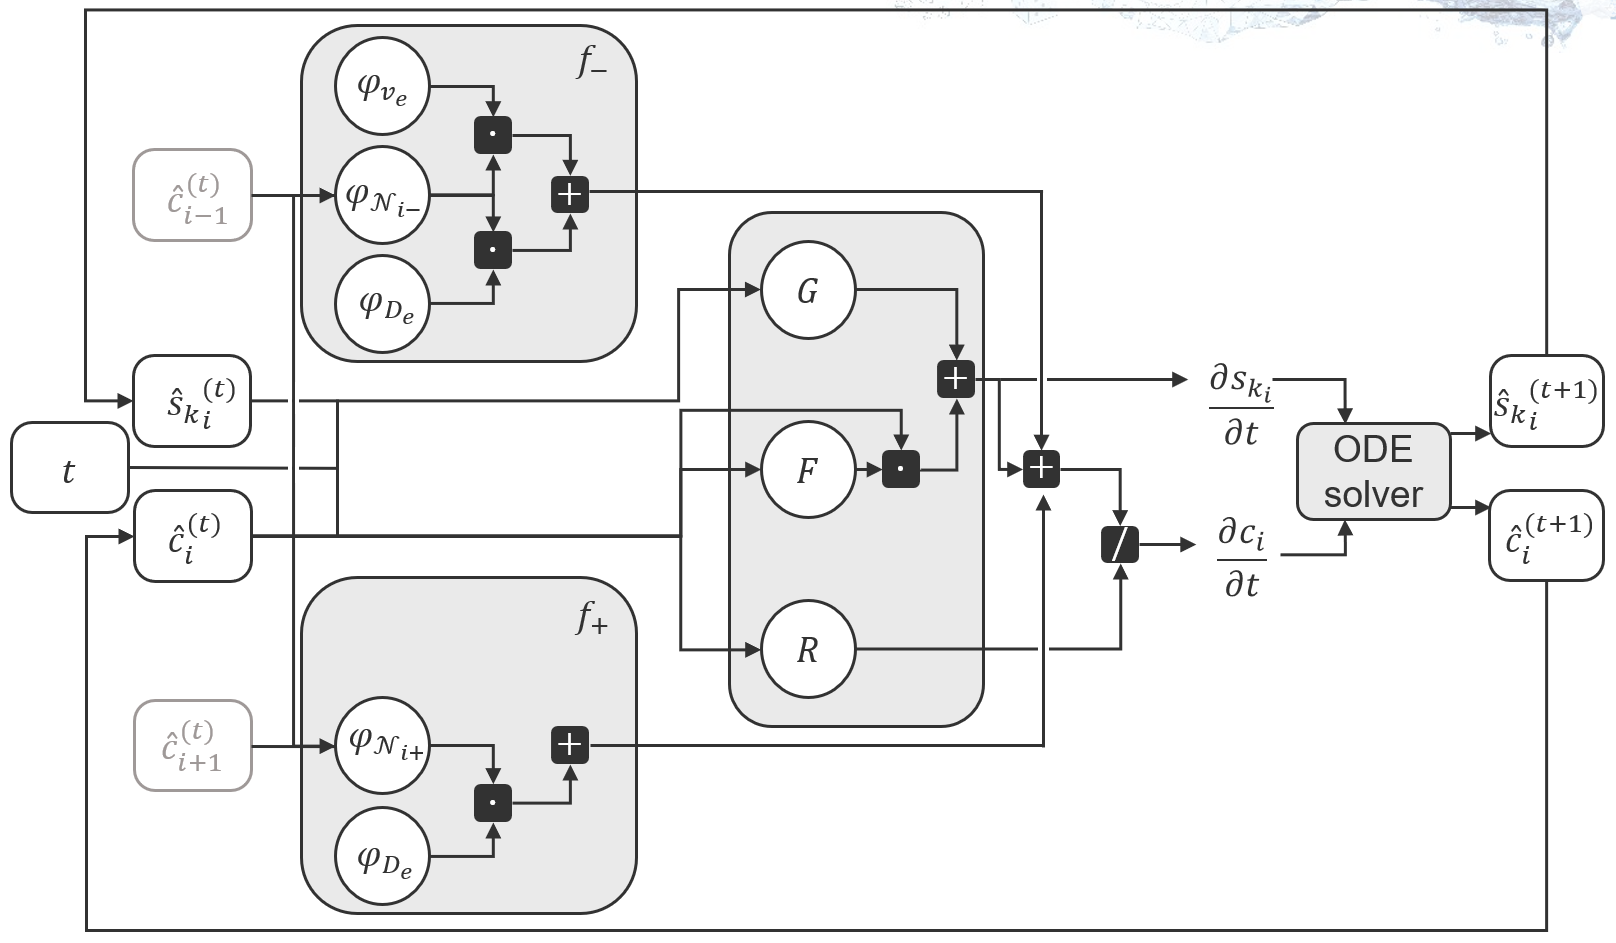
\includegraphics[width=\textwidth]{images/ov_embedding.png}
    \caption[Overview of FINN extensions]{Overview of FINN extensions of this work. In this case learnable functions depended explicitly on time.}
    \label{fig:ovembedding}
\end{figure}
\FloatBarrier
\subsection{Training and Testing}
Generally the training and testing of FINN predicted models is either based on a synthetic solution or scarce experimental data. In each of the following procedures PyTorch's \texttt{Adams} algorithm \cite{Kingma2014Dec} was chosen as optimizer (Listing \ref{code:Adam}). The learning rate is also set in the \texttt{config} .json-file and was partly reduced manually with progressing training epoch number. An automated learning rate schedule was not developed.
\begin{lstlisting}  [float, language=python, caption={Using Adams algoritm for loss calculation.}, label=code:Adam]
# Set up an optimizer and the criterion (loss)
optimizer = th.optim.Adam(model.parameters(), lr=config.training.learning_rate)
\end{lstlisting}
\\
\\
\textbf{Synthetic Data}\\
Training with synthetic data was done either with the entire solution $c(t,x)$, $s_k(t,x) \quad \forall t,x \in \Omega_t \times \Omega_x$ or based on one quarter of the total simulation time to do so-called \textit{in-dis-tests}, in which the learned model is tested with the remaining part of the data set, to assess the extrapolation ability of FINN.\\
In the first case no testing was performed and the Mean Squared Error Loss (MSE) with respect to the FD solution of the entire data set was used. With this setup, model parameters were found.\\
In the second case, again the MSE with respect to the first quarter of the FD solution was used as loss function during training. Calculating the MSE of the entire data set after the test pass resulted in the accuracy of extrapolation of FINN.\\
Generally for MSE loss calculation PyTorch's functionality can be used (Listing. \ref{code:MSE_synt_all}). With the keyword \texttt{mean} the loss is divided by the total number of data points $N$, which is
\begin{equation}
    N = X_{STEPS} \cdot T_{STEPS} \cdot 2.
\end{equation}
For each discretized location and time, $N$ or $\frac{N}{4}$ values including $c$ and $s_k$ are available, respectively.
\begin{lstlisting}  [float, language=python, caption={Using MSE Loss in PyTorch, u: FD solution, u\_hat: FINN approximation.}, label=code:MSE_synt_all]
mse = nn.MSELoss(reduction="mean")(u_hat,u)
\end{lstlisting}
\\
\\
\textbf{Usage of Experimental Data}
\\
In order to include experimental data, the value of the key \texttt{expdata} in \texttt{config} .json-file can be set to \texttt{true}. Using Panda's \texttt{read\_excel} method, the Excel sheet provided by Bierbaum et al. \cite{Bierbaum2022Mar} was read in and converted to a Pandas Dataframe. The data set contains all experimental data of the 4 column experiments (N1\_1 - N1\_4).\\
As mentioned in the introduction chapter, the column was flushed with water for approximately 150 days in each experiment. Water that flew out of the column was collected in an empty container until a specific time, then the concentrations of different PFAS were measured, the container was emptied, and the process was repeated for irregular time increments. Thus, in a measurement at one point in time, all PFAS have accumulated since the previous measurement. Hence, the measurement approximates the outflow concentration at the point in time between the current and previous measurement. To perform this half time step shift, the PFAS concentration in the outflow of the column at the beginning of the experiment was added ($0\frac{\mu g}{g}$), and then the measurement results were assigned to the mean times between two measurements (Fig. \ref{fig:exp_btc}). This data was then used in the loss calculation.
\begin{figure}
	\centering
	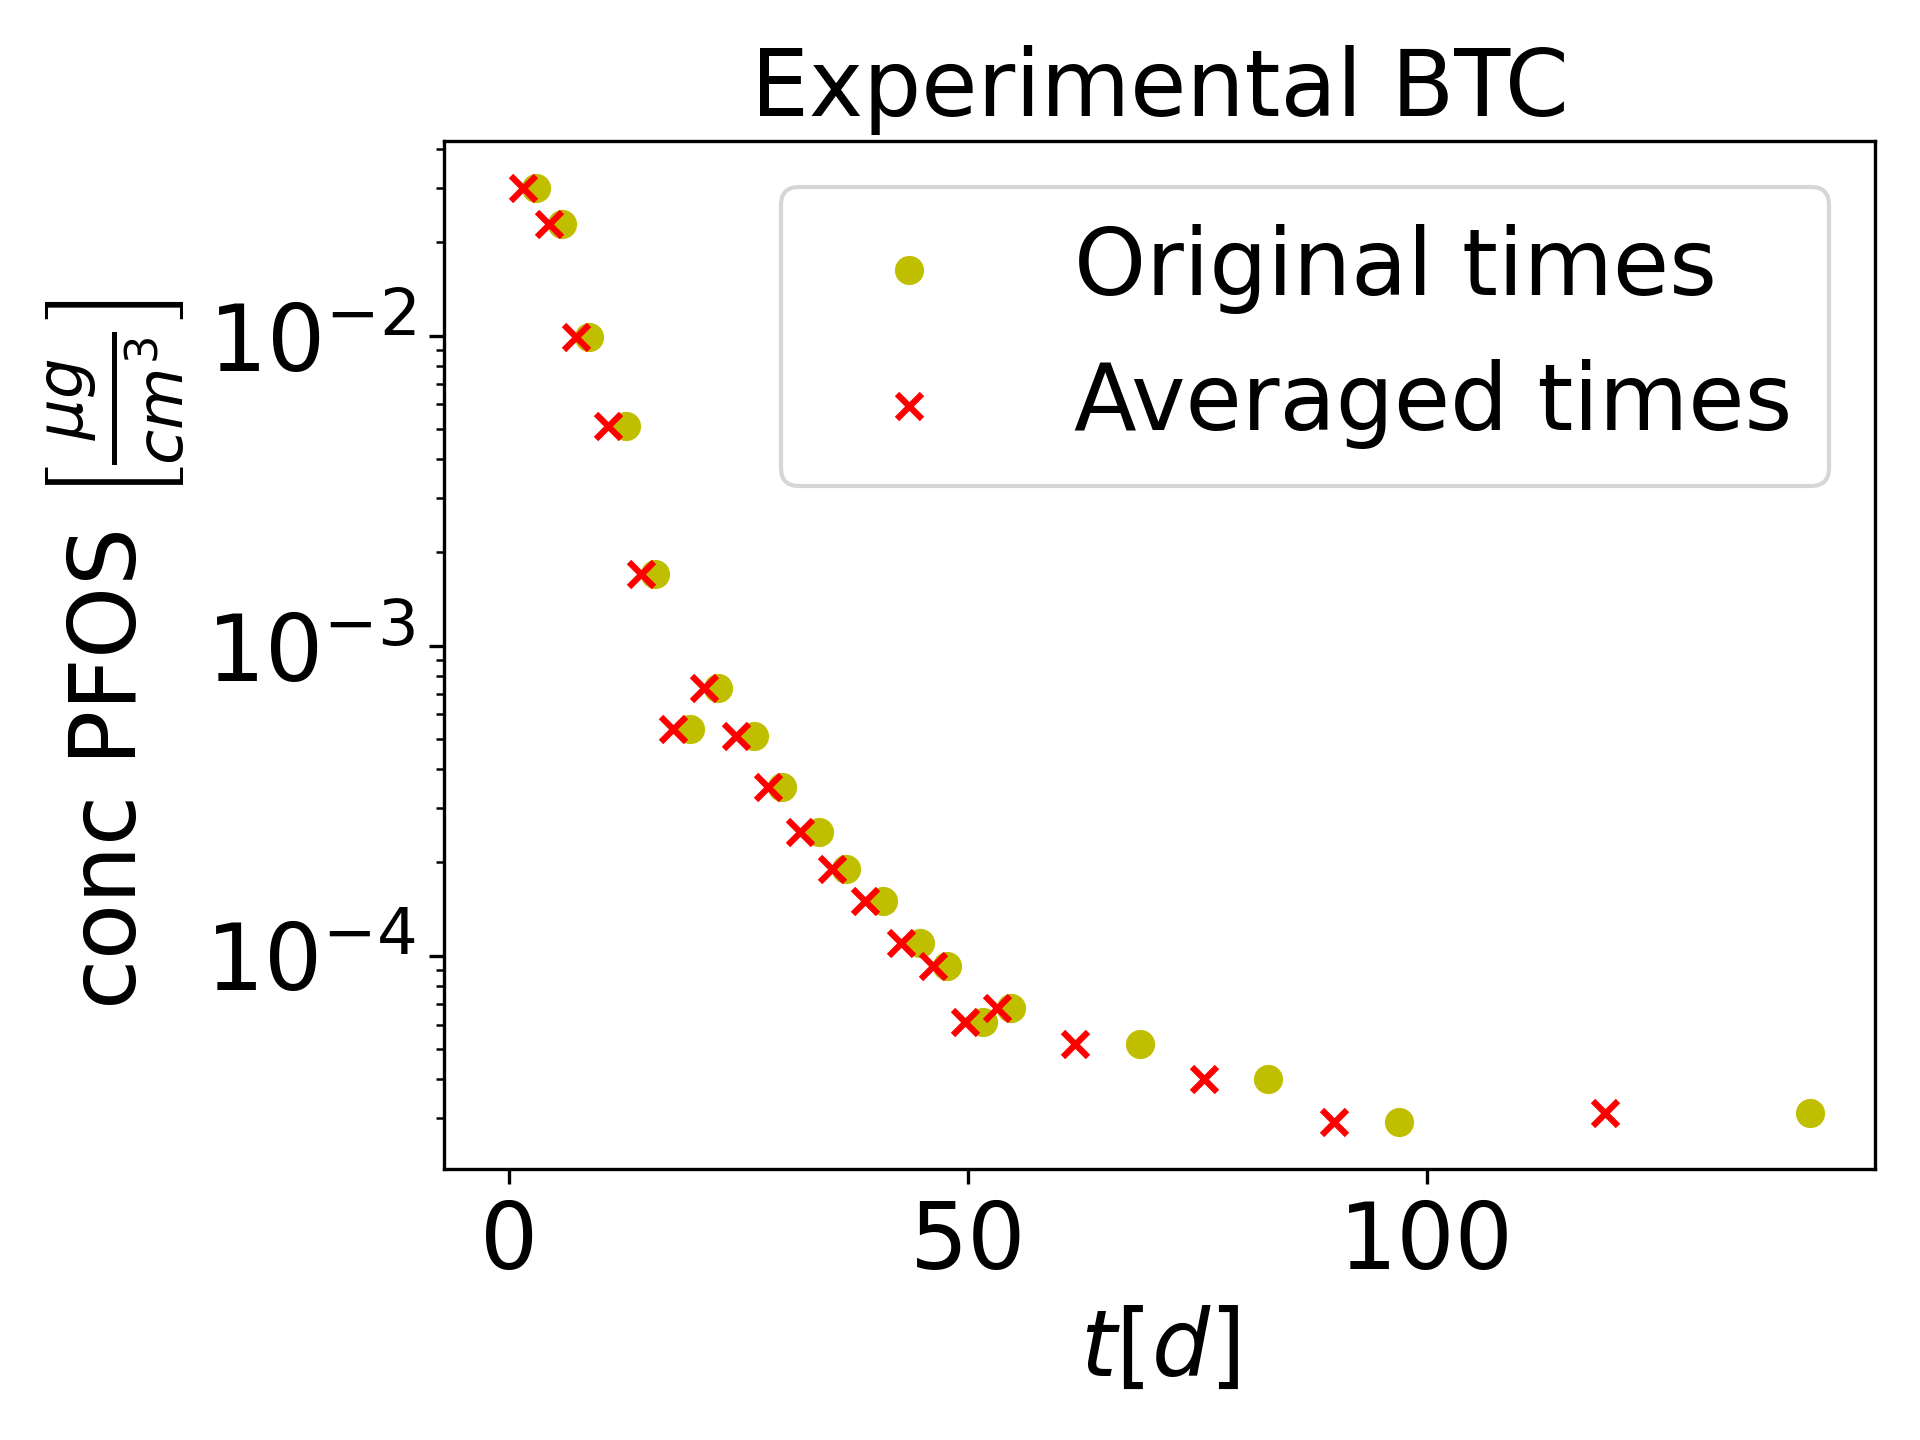
\includegraphics[scale=0.6]{images/exp_btc.png}
\caption[Experimental BTC]{BTC of experiment N1\_1, original data points (green), data points averaged over time (red).}
\label{fig:exp_btc}
\end{figure}
\\
In addition, the total concentrations of PFAS sorbed in the soil at the end of the experiment were investigated. They were approximately homogeneously distributed over the entire column.\\
\\
\textbf{Calculation of Initial Conditions based on Experimental Data}
\\
In order to solve the PDE initial conditions are needed. For an arbitrarily chosen homogeneously distributed $\tilde{c}(t=0)$ the initial condition for $\tilde{s}_k(t=0)$ $\forall x \in \Omega_x$ was calculated using mass conservation
\begin{equation}
    \tilde{m}_{tot} = \tilde{m}_{leached} + \tilde{m}_{end} \overset{!}{=} \tilde{c}(t=0) \frac{V}{m_{soil}} +  \tilde{s}_k(t=0) +\tilde{s}_e(t=0).
    \label{eq:mass_cons}
\end{equation}
$\tilde{m}_{tot}$ $[M M^{-1}]$ is the total initial mass concentration of PFOS in soil, $\tilde{m}_{leached}$ $[M M^{-1}]$ is the mass concentration of PFOS collected in the container at the outflow and $\tilde{m}_{end}$ $[M M^{-1}]$ the sorbed mass concentration at the end of the experiment. These values were measured by the experimentalists. Since the soil was soaked in water before the experiment started, $\tilde{m}_{tot}$ can also be calculated using $\tilde{c}(t=0)$, the cavity volume of the column $V$ $[L^3]$, the soil mass $m_{soil}$ $[M]$, the unknwon $\tilde{s}_k(t=0)$ and $\tilde{s}_e(t=0)$ $[M M^{-1}]$, which is the the initial instantaneously sorbed concentration. $\tilde{s}_e(t=0)$ can be calculated using the Freundlich isotherm and model parameters optimized by Bierbaum et al. $V$ was calculated with
\begin{equation}
    V = \pi \left(\frac{d}{2}\right)^2 n_e h,
\end{equation}
$h$ $[L]$ is the length of the column and $d$ $[L]$ the diameter.\\
Since the choice of $\tilde{c}(t=0)$ is directly coupled to $\tilde{s}_e(t=0)$, $\tilde{c}(t=0)$ must not be chosen too large. Physically, it also makes sense to choose $\tilde{c}(t=0)$ in the order of magnitude of the first measured concentration at the outflow.
\\
\\
\textbf{Loss Calculation for Experimental Data}
\\
Bierbaum et al. optimized manually model parameters for given experimental data. In order to reproduce this work with FINN, in particular the parameter $f$ as ratio between kinetically sorbed and instantaneously sorbed concentration was learned. Several efforts were made to find an accurate loss function.\\
Since the BTC data is log-scaled, a basic MSE as loss function focusses on fitting data points with relatively large orders of magnitude and neglects deviations of concentrations especially at the end of the experiment, where concentrations with significantly smaller orders of magnitude occurred. An appropriate loss function turned out to be the mean squared logarithmic loss of the data points, in order to have the same order of magnitude between the FINN calculated $\hat{c}$ and the experimental $\tilde{c}$ at experimental measurement times $\tilde{\Omega}_t$
\begin{equation}
    L_{I}(\tilde{c},\hat{c}) = \frac{1}{|\tilde{\Omega}_t|-1}\sum_{i=1}^{|\tilde{\Omega}_t|} \left[\log\tilde{c}(t_i,x = X_{STEPS}) - \log\hat{c}(t_i, x=X_{STEPS})\right]^2,
    \label{eq:LI}
\end{equation}
with $t_i \in \tilde{\Omega}_t$. Previously the $\hat{c}$ and $\tilde{c}$ were rescaled by multiplying by $10^{5}$ so that each value is greater than 1. Due to the initial condition at $t = 0$ (and $x = X_{STEPS}$) $\tilde{c}$ and $\hat{c}$ are the same. Thus no loss calculation is needed for this value.
\\
\\
When learning functional relations, $\hat{c}$ and $\hat{s}_k$ can take values of various orders of magnitude (a) as well as negative values (b). A fixed scaling and subsequent logarithmization of the values is not possible. Therefore, to solve problem (a) the averaged sum of the relative L1 error was used as the loss function
\begin{equation}
    L_{II}(\tilde{c},\hat{c}) = \frac{1}{|\tilde{\Omega}_t|-1}\sum_{i=1}^{|\tilde{\Omega}_t|} \frac{|\tilde{c}(t_i,x = X_{STEPS}) - \hat{c}(t_i, x=X_{STEPS})|}{\tilde{c}(t_i,x = X_{STEPS})}.
    \label{eq:LII}
\end{equation}
To solve problem (b) a loss penalty was introduced. Let therefore $\mathbb{O}$ be a tensor containing zeros with the dimensions $X_{STEPS} \times T_{STEPS} \times 2$. And
\begin{equation}
    \hat{u}_{neg} := ReLU(-\hat{u}),
\end{equation}
where $\hat{u}$ is the previously described stacked $\hat{c}$, $\hat{s_k}$ FINN predicted solution. The loss penalty was then calculated with
\begin{equation}
    L_{III}(\mathbb{O},\hat{u}) = 10^5 \cdot MSE(\hat{u}_{neg}, \mathbb{O}).
    \label{eq:LOSS_pen}
\end{equation}
Thus, the more negative $\hat{c}$ and $\hat{s_k}$ are, the larger the loss value becomes. The scaling factor was determined manually. Eqs. \ref{eq:LII} and \ref{eq:LOSS_pen} lead ultimately to the applied loss function for learning functional relations on experimental data
\begin{equation}
    L(\tilde{u}, \hat{u}) = L_{II}(\tilde{c},\hat{c}) + L_{III}(\mathbb{O},\hat{u}).
    \label{eq:loss_exp_func}
\end{equation}
\\
By learning functional relations for experimental data it makes also sense to asses the ability of FINN to learn relations out of initial distributions (\textit{out-dis-tests}). Therefore a model for the functional relations is trained based on experimental data N1\_1 and then tested with experimental data N1\_3, where other parameters occured. In particular the Darcy flux, the mass density, and observed simulation time deviated from the experimental training data set, and were changed before forward passing the trained model. The loss was then calculated using the measurement time points of the new experiment N1\_3 and eq. \ref{eq:loss_exp_func}.\\ 
\\
In order to reproduce this work the following repositories were created: Fork of FINN including comprehensive embedding of 2SS model and DNN models trained with synthetic data \cite{FINN_fork}, source code for DNN models trained with experimental data on high-performance cluster \cite{FINN_emma} and Hydrus files for validation \cite{Hydrus_BA}.